% !TEX encoding = UTF-8 Unicode
\documentclass[
10pt,
aspectratio=169,
]{beamer}
\setbeamercovered{transparent=10}
\usetheme[
%  showheader,
%  red,
  purple,
%  gray,
%  graytitle,
  colorblocks,
%  noframetitlerule,
]{Verona}

\usepackage[T1]{fontenc}
\usepackage[utf8]{inputenc}
\usepackage{lipsum}
%%%%%%%%%%%%%%%%%%%%%%%%%%%%%%%
% Mac上使用如下命令声明隶书字体,windows也有相关方式,大家可自行修改
%\providecommand{\lishu}{\CJKfamily{zhli}}
%%%%%%%%%%%%%%%%%%%%%%%%%%%%%%%
\usepackage{tikz}
\usetikzlibrary{fadings}
\usetikzlibrary{shapes.geometric}
\usetikzlibrary{positioning}
%\tikzset{
%  every overlay node/.style={
%    draw=black,fill=white,rounded corners,anchor=south west,
%  },
%}
% Usage:
% \tikzoverlay at (-1cm,-5cm) {content};
% or
% \tikzoverlay[text width=5cm] at (-1cm,-5cm) {content};
%\def\tikzoverlay{%
%   \tikz[baseline,overlay]\node[every overlay node]
%}%
\tikzset{
  every overlay node/.style={
    anchor=north west,
  },
}
\def\tikzoverlay{%
   \tikz[baseline,overlay]\node[every overlay node]
}%


\newenvironment{smallgreentext}{\scriptsize\color{green}}{\par}
\newenvironment{smallbluetext}{\scriptsize\color{blue}}{\par}
\def\checkmark{\tikz\fill[scale=0.4](0,.35) -- (.25,0) -- (1,.7) -- (.25,.15) -- cycle;}

%
%\setbeamertemplate{sections/subsections in toc}[ball]
%\usepackage{xeCJK}
\usepackage{adjustbox} % Shrink stuff
\usepackage{listings}
\usepackage{caption}
\usepackage{subcaption}
\usefonttheme{professionalfonts}
\def\mathfamilydefault{\rmdefault}
\usepackage{amsmath}
\usepackage{multirow}
\usepackage{booktabs}
\usepackage{bm}
\setbeamertemplate{section in toc}{\hspace*{1em}\inserttocsectionnumber.~\inserttocsection\par}
\setbeamertemplate{subsection in toc}{\hspace*{2em}\inserttocsectionnumber.\inserttocsubsectionnumber.~\inserttocsubsection\par}
\setbeamerfont{subsection in toc}{size=\small}
\AtBeginSection[]{%
	\begin{frame}%
		\frametitle{Outline}%
		\textbf{\tableofcontents[currentsection]} %
	\end{frame}%
}

\AtBeginSubsection[]{%
	\begin{frame}%
		\frametitle{Outline}%
		\textbf{\tableofcontents[currentsection, currentsubsection]} %
	\end{frame}%
}

\title{Comunicaci\'on y socializaci\'on de los resultados}
\subtitle{Escritura, revisi\'on y publicaci\'on de art\'iculos}
\author[L.M.]{Luis Alejandro Morales, Ph.D.}
\mail{email: lmoralesm@unal.edu.co \\ url: \url{https://lamhydro.github.io}}
\institute[UNAL]{Facultad de Ingenier\'ia, Departamento de Ingenier\'ia Civil y Agr\'icola\\
Universidad Nacional de Colombia, Bogot\'a}
\date{\today}
\titlegraphic[width=3cm]{logo_01u}{}

%%%%%%%%%%%%%%%%%%%%%%%%%%%%%%%%
% ----------- 标题页 ------------
%%%%%%%%%%%%%%%%%%%%%%%%%%%%%%%%
% New commands
\newcommand{\gi}{\texttt{Git}}
\newcommand{\gih}{\texttt{GitHub}}
\newcommand{\co}[1]{\alert{\textbf{\large \texttt{#1}}}}

\begin{document}

\maketitle

%%% define code
\defverbatim[colored]\lstI{
	\begin{lstlisting}[language=C++,basicstyle=\ttfamily,keywordstyle=\color{red}]
	int main() {
	// Define variables at the beginning
	// of the block, as in C:
	CStash intStash, stringStash;
	int i;
	char* cp;
	ifstream in;
	string line;
	[...]
	\end{lstlisting}
}
%%%%%%%%%%%%%%%%%%%%%%%%%%%%%%%%
% ----------- FRAME ------------
%%%%%%%%%%%%%%%%%%%%%%%%%%%%%%%%

%----
\section{Generalidades}

\begin{frame}{¿Como obtener ideas para un articulo?}
\begin{itemize}
\item Lectura rápida
\item Vincular ideas cuyas conexiones no fueron previamente establecidas 
\item Usar analogías para sugerir pistas e hipótesis. Esto ayuda a comprender fenómenos y sucesos que no podemos ver
\end{itemize}
\centering
\alert{"Para tener una buena idea, necesitas tener un muchas ideas"} \emph{Jeff McDonnell}
\end{frame}

\begin{frame}{¿Porque escribir y publicar un articulo?}
\begin{itemize}
\item En cumplimiento de realizar un doctorado, resultados y cooperación en un proyecto.
\item Contribuir al estado del arte del conocimiento, ayudar a otros para que puedan desarrollar su trabajo, ayudar a resolver problemas en beneficio de la sociedad.
\item Conseguir un trabajo, triunfar en el mundo académico, convertirse en alguien influyente, etc.
\item Escribir no es simplemente comunicar ideas, es sobre todo cambiar las ideas del lector. 
\end{itemize}
\end{frame}

%\begin{frame}{¿Estrategias para publicar?}
%\begin{columns}
%\column{0.6\textwidth}
%\begin{enumerate}
%
%\end{enumerate}
%\column{0.4\textwidth}
%
%\end{columns}
%\end{frame}




\section{Pasos para la escritura de un articulo}
\begin{frame}{Pasos para la escritura de un articulo}
\begin{enumerate}
\item Escoger la revista para publicaci\'on.
\item Estructurar el paper y escribirlo.
\item Enviar el articulo para revisi\'on (peer review).
\item Si el articulo es aceptado, hacer las correcciones sugeridas y enviarlo de nuevo. En caso de no ser aceptado, revisar y enviarlo a otra revista.
\item Proofreading y publicación.
\end{enumerate}
\end{frame}

\begin{frame}{Pasos para la escritura de un articulo}
Otra visi\'on:
\begin{enumerate}
\item Construya una historia: Extraiga la esencia, pregunta de investigación, hipótesis, figuras claves
\item Organice su historia: Estructure la historia, motivación, bibliografía clave
\item Visualize su historia: Tipos de figuras, colores, formatos
\item Escriba su historia: Adicione contenido a las secciones de la estructura, inicie por lo m\'as sencillo (e.g. Metodología), itere varias veces
\item Revise su historia: Asuma la perspectiva del revisor (evidencia faltante, lógica, fluidez, redundancia, coherencia), pide retroalimentaci\'on
\item Envie su historia
\end{enumerate}
\end{frame}

\begin{frame}{1. Escoger la revista de publicación}
\begin{itemize}
\item Esta decisi\'on es muy importante porque el \alert{impacto} y el \alert{alcance} de su art\'iculo depende en gran medida de la revista en donde se publique. 
\item Se escribe el art\'iculo siguiendo las directrices de la revista en cuanto
\item Es importante analizar cada aspecto de la revista como:
\begin{itemize}
\item Factor de impacto.
\item Pertinencia del tema y audiencia.
\item Modalidad de publicaci\'on.
\item Limitaciones de numero de paginas, caracteres.
\item Costos de publicación (acceso abierto o de pago).
\end{itemize}
\item Es aconsejable hablar con su supervisor, profesores y colegas. 
\item De acuerdo con las referencias citadas en el articulo, la revista m\'as es seria la mas recomendada.
\item Experiencia previa suya o de su supervisor con una revista determinada.
\end{itemize}
\end{frame}


\begin{frame}{1. Escoger la revista de publicación}
\centering
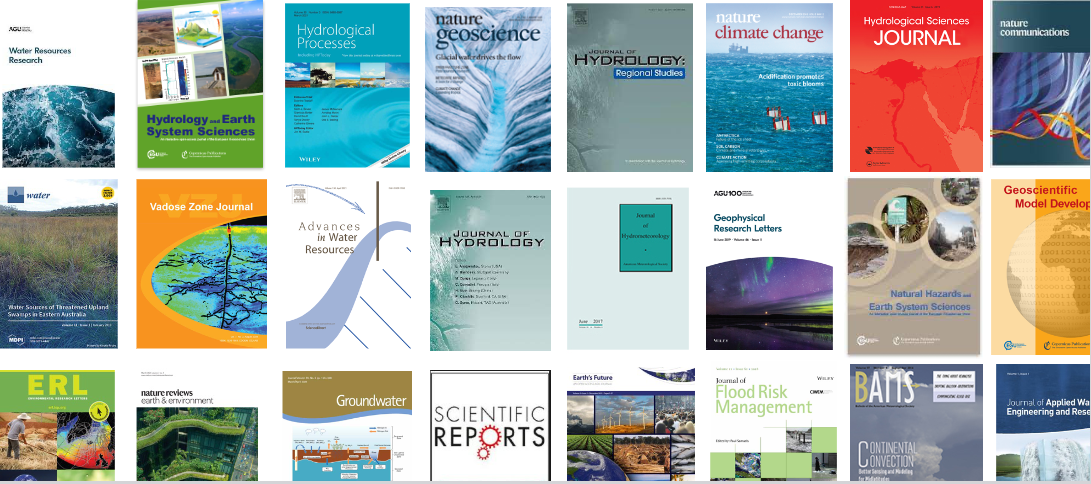
\includegraphics[width=\textwidth]{fi2.png}
\end{frame}


\begin{frame}{2. Estructurar el paper y escribirlo: Estructura}
Una estructura típica es la siguiente (no para artículos de revisi\'on):
\begin{columns}
\column{0.3\textwidth}
\begin{enumerate}
\item T\'itulo
\item Resumen
\item Introducci\'on
\item Metodolog\'ia y materiales
\item Resultados
\item Discusi\'on
\item Conclusiones
\end{enumerate}
\column{0.7\textwidth}
\centering
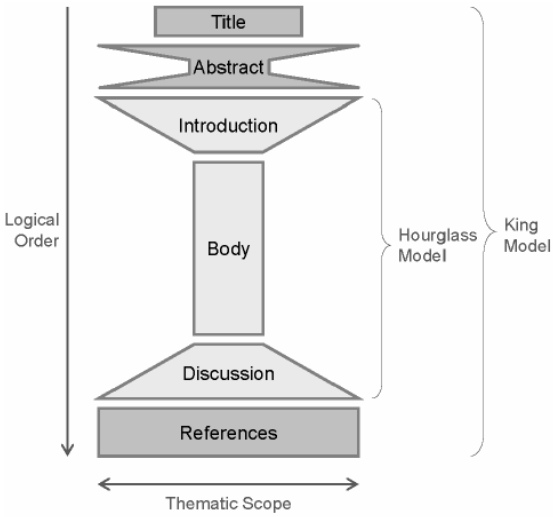
\includegraphics[width=0.74\textwidth]{fi1.png}
\end{columns}
\end{frame}

\begin{frame}{2. Estructurar el paper y escribirlo: Escritura}
\begin{enumerate}
\item Identificar/definir qué hay de nuevo y escribir los puntos claves. Debe reflejarse en el título
\item Defina qué pregunta de investigación está respondiendo.
\item Escriba el resumen (puede cambiar, pero ayuda a definir la historia del artículo, sabe a donde va, no se pierde)
\item Desarrollar la estructura del artículo (según la historia), incluyendo subsecciones, viñetas y figuras.
\item Sección de métodos (esto es fácil ya que sabe exactamente lo que ha hecho, ayuda para quitarle el miedo a la página en blanco)
\item Sección de resultados - sigue el esquema y el orden de las figuras. 
\item Resultados: describa el resultado de sus análisis, lo más cuantitativo posible. Sin especulaciones
\item Discusión: interprete sus resultados, combine diferentes resultados (algunas especulaciones está bien si se indica claramente), relacione sus resultados con el conocimiento disponible.
\item Conclusiones (evite el resumen): escriba lo que se encontr\'o de sus resultados.
\item Introducción: no escriba sobre el tema general, sino resuma lo que es conocido sobre la pregunta de investigación (la introducción y la discusión deben ser coherentes)
\end{enumerate}
\end{frame}


\begin{frame}{The top-down approach}
\begin{enumerate}
\item Presenta la historia:
\begin{itemize}
\item ¿Cuál es el status quo?
\item ¿Qué esta mal en el status quo?
\item ¿Cómo este art\'iculo va m\'as all\'a o mejora el status quo?
\end{itemize}
\item Desarrollar un esquema con títulos y subtítulos
\item Repita esto muchas veces, agregando sub-sub-encabezados
\item Identifique figuras clave para contar la historia.
\item Los subtítulos se convierten en el tema para párrafos.
\item Asignar tareas de escritura a coautores, !divide y vencerás!.
\end{enumerate}
\end{frame}

\begin{frame}{The top-down approach}
No empieces a escribir hasta que:
\begin{itemize}
\item La estructura es sólida como una roca
\item Las figuras están listas
\item Subtítulos = temas de párrafo
%\item Cada sección se asigna a la novedad/necesidad imperiosa de este artículo en la revista literatura
\end{itemize}
\end{frame}

\begin{frame}{El titulo, el resumen y las figuras}
\begin{itemize}
\item \alert{T\'itulo}:Genere una buena primera impresi\'on con el t\'itulo con de acuerdo con el mensaje principal de su art\'iculo.
\begin{itemize}
\item \alert{On comparing streamflow and groundwater heads}
\item \alert{A systematic comparison of streamflow and groundwater heads across the USA}
\item {\color{blue}Widespread potential  loss  of streamflow into underlying aquifers across the USA}
\end{itemize}
\item \alert{Resumen}: Genere una buena primera impresi\'on haciendo énfasis en lo que ha descubierto y por que esto es importante. El resumen debe responder las siguientes preguntas:
\begin{itemize}
\item ¿Que fue lo que se hizo?
\item ¿Por qué se hizo?
\item ¿Cómo se hizo?
\item ¿Qué se encontró?
\item ¿Cuál es la importancia de los hallazgos?
\end{itemize}
\item \alert{Figuras}: Genere una buena primera impresi\'on con figuras que claramente muestren un mensaje (e.g. mensaje principal) y que tenga un formato. 
\end{itemize}
\end{frame}


\begin{frame}{¿Porque los artículos de investigaci\'on son rechazados?}
\centering
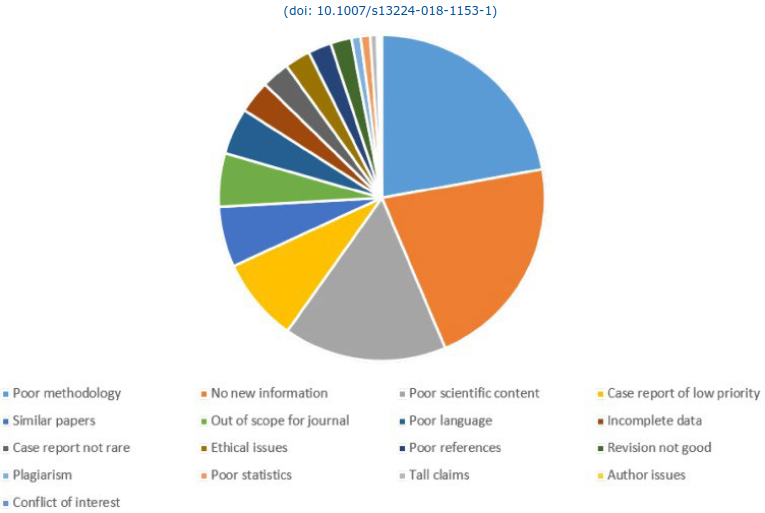
\includegraphics[width=0.73\textwidth]{fi3.png}
\end{frame}

\begin{frame}{3. Revisi\'on del articulo}
\begin{enumerate}
\item Decisión del editor
\begin{itemize}
\item Con o sin revisión
\begin{itemize}
\item Apropiado para la revista
\item Novedoso y general
\item Las conclusiones son soportados por los resultados y la discusión
\end{itemize}
\item Revisión
\begin{itemize}
\item Algunos son superficiales
\item Agresivos
\item Precisos y útiles
\end{itemize}
\end{itemize}
\item Después de leer la revisi\'on, tómese un tiempo antes de reaccionar.
\item Reenvie el articulo 
\begin{itemize}
\item Diferente revista
\begin{itemize}
\item Pueden ser los mismos revisores
\item Mejor incluir las observaciones de la revisión anterior
\end{itemize}
\end{itemize}
\end{enumerate}
\end{frame}

\begin{frame}{3. Revisi\'on del articulo}
\centering

\includegraphics[width=0.7\textwidth]{fi4.png}
\end{frame}

\section{Otros aspectos}
\begin{frame}{Tener en cuenta que el lector es lo m\'as importante}
\begin{itemize}
\item Tu trabajo debe cambiar como el lector ve el mundo.
\item Comunique tu mensaje principal el en \alert{titulo},   \alert{resumen} y \alert{figuras}.
\item Una vez las condiciones anteriores se cumplan, podemos preocuparnos por los detalles de la escritura.
\item Haz la "vida" del lector tan fácil como sea posible.
\end{itemize}
\end{frame}

\begin{frame}{Tener en cuenta que el lector es lo m\'as importante}
\begin{enumerate}
\item Publicar es emocionante, satisfactorio y extremadamente importante para una carrera académica
\item Un resultado científico sólo "existe" cuando se publica
\item Intenta siempre publicar en la mejor revista posible (no tomes un rechazo como algo personal, intenta aprender de ello y vuelve a intentarlo)
\item Adopte la perspectiva del lector. ¿Por que resulta útil aprender de este estudio? (sea lo más cuantitativo posible)
\item Apunta a un mensaje claro.
\item Se ofrecen cursos de "escritura científica" en casi todas partes, tome ventaja de ellos.
\item Escribir un artículo es una habilidad, por lo que es fácil pero requiere algo de práctica (Günther Blöschl 2011)
\end{enumerate}
\end{frame}

\begin{frame}{1 hora de escritura diaria}
\begin{itemize}
\item Te ayuda a sentir que has logrado “algo” ese día
\item Te mantiene "en forma" y "en condiciones"
\item Mantiene lo principal, lo esencial
\item Reconoce que se el trabajo profundo es el mejor
\item En cualquier deporte hay que mantenerse tonificado y acondicionado.
\item Si pierdes la práctica, rápidamente pierdes fitness, y escribir y editar se vuelven mas laboriosos
\item Entonces, aunque abundan las distracciones, proteja ese 'entrenamiento' diario en el teclado
\end{itemize}
\end{frame}

\end{document}



